\section{Further Defense Mechanisms}
\label{sec:defences}
Beyond StruQ and secAlign, there are many other defense mechanisms which aren't based on model fine-tuning. 
These defenses instead rely solely on enforcing security architecturally.
In this chapter three such approaches will be discussed in detail.
\subsection{F-secure LLM Systems}
One such system is the f-secure LLM system, a representative framework based on Information Flow Control (IFC) \parencite{wu2024systemlevel}.
This system separates the application into 3 parts.
Upon receiving a prompt it first is given to the LLM-planner, which generates execution steps based on the query as well as the previous steps.
These steps are then each given to the Rule-based Executor, which initiates a new LLMs instance to complete the query based on the generated steps from the planner.
During the execution the Security Monitor overlooks the entire process, checking both the generated steps from the planner and the output of the LLM instance for suspicious/ incorrect content. 
It does this by adding labels for untrusted and trusted information, and then ensuring that the planner only has access to trusted information, when generating the steps the actual LLM-model has to follow \parencite{wu2024systemlevel}. 
\begin{figure}
    \begin{center}
        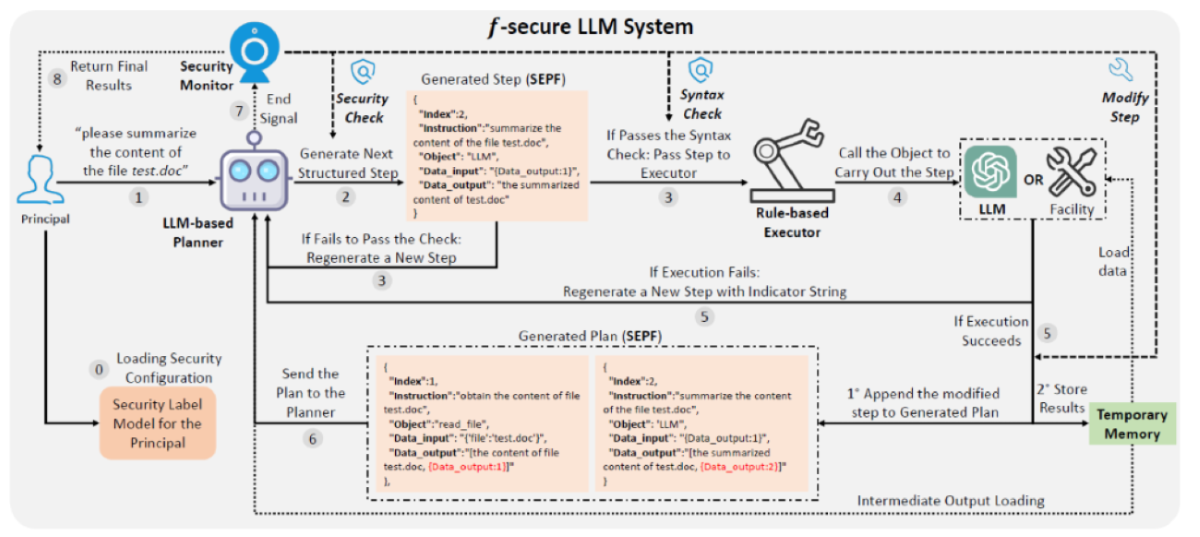
\includegraphics{./images/fsecure}        
    \end{center}
    \caption{Architecture of an f-secure LLM system \parencite{wu2024systemlevel}}
\end{figure}
\subsection{Agent Security}
In the domain of agentic systems RTBAS (Robust Tool-Based Agent System) and CaMeL (Capabilities for Machine Learning) provide specialized protections for tool-calling scenarios.
RTBAS employs dependency screening to identify which parts of a model's history are relevant for generating a tool call.
It uses "LM-as-a-judge" or attention-based screeners to mask irrelevant regions and selectively propagate security metadata, preventing unnecessary "tainting" of tool calls while maintaining utility\parencite{zhong2025rtbas}.\\
Similarly, CaMeL extracts control and data flows from queries as pseudo-Python code and uses a custom interpreter to enforce capability-based policies.
By assigning unforgeable tags (capabilities) to every value, the system can block tool execution—such as sending an email—if private data is passed to unauthorized recipients, regardless of what an injected prompt might command \parencite{debenedetti2025defeating}.\\
\subsection{Regular Defenses}

